\documentclass[preprint,superscriptaddress]{revtex4-1}
%\documentclass[twocolumn,superscriptaddress]{revtex4}


\usepackage{amsmath} 
\usepackage{amssymb} 
 \usepackage{amsfonts}

\usepackage{graphicx} 

\usepackage{array}
\usepackage{multirow}
\usepackage{color}
\usepackage{transparent}
\usepackage{float}

\newcommand{\vect}[1]{\boldsymbol{\mathbf{#1}}}



\begin{document}

\bibliographystyle{apsrev4-1} 


\title{Diffusion-Controlled Reactions over Fluctuating Barriers} 

\author{Jakob J. Kolb}
\affiliation{Institut f{\"u}r Physik, Humboldt-Universit{\"a}t zu Berlin, Newtonstr.~15, 12489 Berlin, Germany}
\author{Stefano Angioletti-Uberti}
\affiliation{Institut f{\"u}r Physik, Humboldt-Universit{\"a}t zu Berlin, Newtonstr.~15, 12489 Berlin, Germany}
\author{Joachim Dzubiella}
\email{joachim.dzubiella@helmholtz-berlin.de}
\affiliation{Institut f{\"u}r Physik, Humboldt-Universit{\"a}t zu Berlin, Newtonstr.~15, 12489 Berlin, Germany}
\affiliation{Soft Matter and Functional Materials, Helmholtz-Zentrum Berlin, Hahn-Meitner Platz 1, 14109 Berlin, Germany}



\begin{abstract}


We investigate the influence of a stochastically fluctuating potential barrier on the diffusion-controlled bimolecular reaction rate
for ideal reactants adsorbed by a spherical sink particle.  The reactive sink is shielded by a step-barrier potential (i.e., a spherical shell)  
whose magnitude stochastically fluctuates between multiple states. For such a minimalistic setup, we derive an implicit analytical 
solution for the resulting Fokker-Planck equation to obtain the diffusion-controlled reaction rate.  We verify the results with direct numerical 
methods as well as Brownian Dynamics computer simulations for a two-state process. As a key result we demonstrate that the two-state 
system exhibits  a resonant  behavior for the diffusion-controlled reaction rate if the {\it fluctuation decay length} is on the order of the system size.  
This {\it resonant reaction} resembles the resonant activation previously observed in thermally activated escape problems 
over fluctuating barriers. We selectively explore the behavior of the resonant reaction in the dependence of barrier potential height, 
barrier geometry (spacing and width), surface reaction rate,  and discuss analytical limiting laws for slow and fast barrier switching. 

\end{abstract}

\maketitle

\section{Introduction}

Bimolecular binding reactions  in liquid solvents are ubiquitous in chemistry and biology and typically involve the crossing of a potential or kinetic barrier during their diffusion-controlled approach \cite{Calef1983, berg1985diffusion}. However, in complex systems that exhibit multiple degrees of freedom these barriers can thermally fluctuate in space and time between multiple states~\cite{Calef1983, berg1985diffusion,kang,zwanzig}. Timely examples are the binding of ligands to conformationally-gated proteins \cite{Szabo1982,greives}, reaction in complex cellular environments~\cite{noe},  or weakly hydrophobic pockets \cite{Setny2013, Mondal2013}, the reactant approach to the active catalytic site in polymer-coated carrier particles \cite{Wu2012a, stefano}, or the association kinetics of biomolecules with fluctuating charges \cite{kirkwood,mikael}. How the diffusion-controlled association rate depends on the barrier fluctuation rate and the details of the fluctuating potential or diffusivity profiles is essentially unexplored. Previous related works almost exclusively focused on fluctuating reactivity rate constants and fluctuating reactive patches ('gates')  on the particle surface~\cite{Calef1983, berg1985diffusion,kang,zwanzig}. The systematic study of thermally fluctuating longer-ranged potentials and diffusivities has been neglected so far, although one can expect significant alteration of binding rates and strong reaction-fluctuation couplings, as indicated by the 'inverse' problem of the diffusional escape over fluctuating potential barriers~\cite{Doering1992, Zurcher1993, Pechukas1994, Reimann1995, Reimann1995a}.\\


Smoluchowski on reaction rates: \cite{Smoluchowski1916, Smoluchowski1917a}. \\
\begin{equation}
    k_S = 4 \pi D R_s.
\end{equation}

Debye theory \cite{Debye1942}
\begin{equation}
    k _{D} =4 \pi D \left\{\int_{R_S}^\infty\frac{\exp(U(r)/k_BT)}{r^2}{\rm d}r\right\}^{-1}.
    \label{SD_rate_slow_intro}
\end{equation}


Here we study the problem of diffusion-controlled reaction rates in the Smoluchowski-Debye sense \cite{Smoluchowski1917a, Debye1942} in the presence of a fluctuating potential barrier. \\
Basics of transition rate theory: experimental\cite{hoff1884, arrhenius1889} and analytic \cite{Kramers1940}. \\
Resonant activation: first observed \cite{Doering1992}, further studied \cite{Zurcher1993, Pechukas1994, Reimann1995, Reimann1995a} \\
Smoluchowski on reaction rates: \cite{Smoluchowski1916, Smoluchowski1917a}. \\
Debye theory \cite{Debye1942}, applications in heterogeneous catalysis, polymer chain growth kinetics, colloid or crystal growth and enzyme ligand binding \cite{hawker2001new, hansen2002robust, aizenberg1999control, achilias1992development, wisanrakkit1990glass, berg1985diffusion, kuo1974studies, richter1974, alberty1958, Wu2012a} corrections corrections due to hydrodynamic interaction between mutually approaching particles \cite{Friedman1966, Wolyes1976}, corrections due to combined hydrodynamic and hard sphere interaction for dilute but finite substrate concentration \cite{Dzubiella2005} and crowding \cite{Dorsaz2010} and other generalizations such as multiple sinks competing for the substrate \cite{Reck1968a, Reck1968b} or setups where the reaction at the sink is limited to a certain reactive patch that covers only a fraction of its surface \cite{schmitz1972role, schurr1976, shoup1981diffusion, shoup1982role}. \\
On the importance of fluctuation in in gating (oxygen binding to hemoglobin)~\cite{perutz1966x, muirhead1967structure, Szabo1978, Szabo1982} 
and PNIPA Yolk shell nano particles \cite{Wu2012a} and hydrophobic cavity-ligand binding \cite{Setny2013, Mondal2013}. \\

\section{Methods} 

\subsection{Model and analytical treatment}

\begin{figure}[H]
\begin{center}
	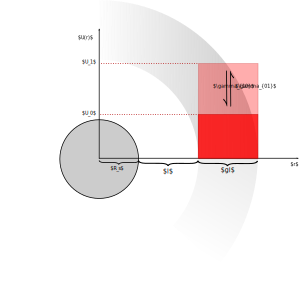
\includegraphics[width = 0.5 \textwidth]{plots/Skizze.pdf}
    \caption{Sketch of our model system consisting of a spherical sink particle (gray sphere) and a fluctuating step-barrier (red). The sink radius is $R_s$, while the barrier is positioned between radial distances $a$ and $b$. The gap between the sink and the  barrier is thus $l=a-R_s$.  The scaled barrier width we then define as $gl=b-a$. In this illustration, the barrier fluctuates between two states (dark and light red) with energies $U_0$ and $U_1$ and transition rates $W_{01}, W_{10}$, respectively.}
\label{fig0}
\end{center}
\end{figure}

Our minimalistic model is illustrated in Fig.~1. As in the classical Smoluchowski-Debye picture for diffusion-controlled reactions~\cite{Smoluchowski1917a, Debye1942},  the diffusional approach of reactants over a barrier to a central, spherical sink with radius $R_s$ is considered.  We set $R_s=1$  as our unit length scale in the remainder of the paper. A step-barrier potential is defined by the piece-wise function 
 \begin{eqnarray}
 U_n(r) = U_n \left[\Theta(r-a)-\Theta(r-b)\right] 
 \end{eqnarray}
where $U_n$ is the barrier height of state $n$, $l=a-R_s$ is its radial distance to the sink surface, and we define the barrier width as $gl=b-a$, 
where $g$ is the ratio between barrier width and the length $l$. Hence, by playing with $g$ for a fixed $l$ we change the barrier width, 
while by playing with $l$ for a fixed $g$ we change both the ratio of barrier spacing and width with respect to the unit scale $R_s$. Hence, keeping $g$ on the
order of unity, $l$ is a convenient measure of system size. 

We now assume that the barrier height switches stochastically between $N$ states according to a discrete time reversible Markov process $\eta(t)$. Therefore the system evolution follows the stochastic differential equation (SDE) 
\begin{equation}
    \frac{{\rm d} \vec{r}}{{\rm d} t} = \vec{\nabla}\frac{1}{\gamma}f(r)\eta(t) + \sqrt{2D}\vec{\varepsilon}(t)
    \label{SDE}
\end{equation}
where $\varepsilon(t)$ is white Gaussian noise with time correlation $\left< \varepsilon(t) \varepsilon(t') \right> = \delta(t-t')$ and $\eta(t) \in [U_0,\cdots U_{N-1}]$ and $f(r) = \Theta(r-a)-\Theta(r-b)$ define the height and shape of the potential barrier. The friction constant $\gamma$ is related to the reactant self-diffusion constant $D$ through the Einstein relation $\gamma = k_BT/D$, where $k_BT$ is the thermal energy.  

Equivalently to the SDE the system can be described in terms of a combined reaction-diffusion equation system for the particle density function $\rho_n(\vec{r},t)$ of the discrete variable $n=0,..,N-1$ of the potential and the continuous variable $\vec{r}$ of the overdamped particles.
The intervals in $r$ with constant potential, namely $R_s \le r < a$, $a \le r <  b$, $r>b$ will be referred to as (I), (II), and (III) in the following. 
The advantage is that such a system can be treated analytically for the case of step-barrier potentials as we will describe in the following. 
The reaction diffusion-equation system can be expressed via
\begin{equation}
    \frac{\partial}{\partial t}\vect{\rho}(\vec{r},t) = \left\{ \mathbb{F} + \mathbb{W} \right\} \vect{\rho}(\vec{r},t)
    \label{mfpe}
\end{equation}
with $\mathbb{F}$ being the Fokker-Planck operator
\begin{equation}
    \mathbb{F} = {\rm  diag}\left[\vec{\nabla} \frac{1}{\gamma} \left(\vec{\nabla} U_n f(r)\right) + D\vec{\nabla}^{2} \right].
    \label{FPO}
\end{equation}
$\mathbb{W}$ is the transition rate matrix of the Markov process for the barrier switching. $\vect{\rho}(\vec{r},t)=(\rho_0(\vec{r},t),\cdots,\rho_{N-1}(\vec{r},t))^{T}$ denotes the vector of particle density functions related to each state of the potential barrier. Since the underlying Markov process of $\mathbb{W}$ is time reversible the transition rate matrix satisfies detailed balance. This also implies that the particle density vector at infinite distance is equal to the equilibrium distribution $\vect{\rho}^{(eq)}$ of $\mathbb{W}$. 

With these prerequisites it is now possible to find a similarity transform $\mathbb{T}_{ij}=[\rho_n^{(eq)}]^{1/2}\delta_{i,j}$ such that the resulting $\mathbb{T}^{-1}\mathbb{W}\mathbb{T} = \mathbb{S}$ is symmetric \cite{Oppenheim1977}. This symmetric matrix can then be diagonalized by an orthogonal transformation $\mathbb{D}$ resulting in $\mathbb{D}^{\dagger}\mathbb{S}\mathbb{D} = - {\rm diag}[\lambda_n]$. It can be shown \cite{VanKampen1992} that $\lambda_{n>0}>0$ and $\lambda_0=0$ with corresponding eigenvector $\mathbb{D}_{0,n}=[\rho_n^{(eq)}]^{1/2}$.   Therefore we can give a steady-state solution $\vect{\rho}(\vec{r}) = \mathbb{T}\mathbb{D}\tilde{\vect{\rho}}(\vec{r})$ to eq.~\eqref{mfpe} in terms of eigenfunctions of $\mathbb{W}$ via
\begin{align}
    \label{solution}
    \tilde{\rho}_{0}^{(j)}(r) &= c_{0,1}^{(j)} + c_{0,2}^{(j)} \frac{1}{r} \\
    \tilde{\rho}_{n \ne 0}^{(j)}(r) &= c_{n,1}^{(j)}\frac{1}{r} \exp\left[-r\sqrt{\frac{\lambda_n}{D}}\right] + c_{n,2}^{(j)}\frac{1}{r} \exp\left[r\sqrt{\frac{\lambda_n}{D}}\right]  \nonumber
\end{align}
separately for the regions (I), (II), and (III) exploiting the fact that the Fokker-Planck operator $\mathbb{F}$ is invariant under the transformations $\mathbb{T}$ and $\mathbb{D}$ for $r\ne a, b$. The coefficients $c^{(j)}_{n,k}$ have to be obtained from boundary and density matching conditions at $r=a,b$. From this solution it is visible that the spatial influence of the potential fluctuations decays with a certain \textit{fluctuation decay length} equal to
\begin{equation}
    r_d = \left\{\sqrt{\frac{\lambda_m}{D}}\right\}^{-1}
    \label{decay_length}
\end{equation}
that only depends on the diffusion constant of the Brownian particles and the largest nonzero eigenvalue $\lambda_m$ 
of the transition rate matrix. In a simple two-state case, as exemplary studied in this work, $\lambda_m$ 
expresses essentially the transition rate between the two states. The decay length describes the mean diffusive path 
of an particle after its disturbance by the fluctuations and thus is a measure for the spatial 
range of the action of the fluctuation.

To derive the matching conditions we use eq.~\eqref{mfpe} which in steady-state is equivalent to
\begin{equation*}
     \frac{1}{\gamma}\rho_n(r) \vec{\nabla} U_n(r) + D \vec{\nabla} \rho_n(r) = \frac{J_n(R_s)}{4 \pi} - \left\{ \mathbb{W} \int_{R_s}^{r} \vect{\rho}(r') {\rm d} r' \right\}_{n}
\end{equation*}
where $J_n$ denotes the flux of particles in state $n$ through the sink surface. This expression is then integrated over a small vicinity of size $\varepsilon$ including the jump discontinuity at $r = a$. Taking the limit of $\varepsilon \rightarrow 0$ results in 
\begin{equation}
    \vect{\rho}^{(I)}(a) = {\rm diag}\left[\exp\left\{\frac{U_n}{k_B T} \right\}\right]\vect{\rho}^{(II)}(a)
    \label{dens_fit1a}
\end{equation}
where $\vect{\rho}^{(I)}(a)$ is the density profile for $r \le a$ and $\vect{\rho}^{(II)}(a)$ is the density profile for $ a<r\le b$ right at the jump discontinuity of the potential barrier (consequently $\vect{\rho}^{(III)}$ denotes the density profile at $b<r$). 
Analogous considerations lead to matching conditions for the the density profile at $r=b$
\begin{equation}
    \vect{\rho}^{(II)}(b) = {\rm diag}\left[\exp\left\{\frac{-U_n}{k_B T} \right\}\right]\vect{\rho}^{(III)}(b)
    \label{dens_fit1b}
\end{equation}
and their derivatives
\begin{equation}
    \vec{\nabla}\vect{\rho}^{(I)}(a) =\vec{\nabla}\vect{\rho}^{(II)}(a) 
    \label{dens_fit2a}
\end{equation}
and
\begin{equation}
    \vec{\nabla}\vect{\rho}^{(II)}(b) =\vec{\nabla}\vect{\rho}^{(III)}(b). 
    \label{dens_fit2b}
\end{equation}
The coefficients $c_{n,i}^{(j)}$ in eq.~(\ref{solution}) are calculated by applying the inverse transform $\vect{\rho}(r) = \mathbb{D}^{\dagger}\mathbb{T}^{-1}\tilde{\vect{\rho}}(r)$ and solving the system of linear equations arising from the fit conditions in eq. \eqref{dens_fit1a}, \eqref{dens_fit1b}, \eqref{dens_fit2a}, \eqref{dens_fit2b} and boundary conditions at $r=R_s$ and $r \rightarrow \infty$. For the Brownian reactants it is assumed that their total density equals the bulk values $\rho_0$ for $r \rightarrow \infty$. Let us also assume for the beginning that they vanish as their trajectory reaches the boundary of the sink at $r = R_s$. That is, we assume fully adsorbing boundary conditions $\rho_n(r=R_s)=0$.  
With that, finally, the diffusion controlled reaction rate over the fluctuating barrier is calculated from $\vect{\rho}^{(I)}$ as
\begin{equation}
    k = 4 \pi D R_s^{2}\sum_n \left. \frac{\partial \rho_n^{(I)}(r)}{\partial r} \right|_{R_s}.
    \label{rate_konstant}
\end{equation}

More generally, it proves also to be interesting to impose a non-perfect sink. In this case the boundary condition at the sink surface is modified as
\begin{equation}
    4 \pi R_s^2 \sum_n \left. \frac{\partial \rho_n^{I}(r)}{\partial r} \right|_{R_s} = k_{\rm surf} \sum_n \left. \rho_n^{(I)}(r) \right|_{R_s}
    \label{nonideal_sink_bc}
\end{equation}
such that the particle flux through the sink surface is proportional to the total particle density (probability) at the sink and
the surface reaction rate $k_{\rm surf}$. 
The full analytical solution for the density profiles and the numerical evaluation of the rates by eqs.~(\ref{rate_konstant}) and ~(\ref{nonideal_sink_bc}) 
was implemented in a script in the Mathematica software~\cite{mathematica} and evaluated for density profiles and rates.

\subsection{Two-state barrier}

The simplest possible setup in the previously developed numerical and analytical framework is that of a two state barrier that switches between one \emph{off} ($U_0 = 0$) and one \emph{on} ($U_1 \ne 0$) state symmetrically, i.e. the \emph{on} $\rightarrow$ \emph{off} and \emph{off} $\rightarrow$ \emph{on} rates are equal:
\begin{equation}
    W_{01}=W_{10}=W
    \label{symmetric_rates}
\end{equation}
This allows for the detailed study of effects solely coming from the coupling of the individual timescales of barrier fluctuations and diffusive transport without any complexity of having a spectrum of timescales. 

The first step for the investigation of the example is the calculation of the analytic solution for the density profiles of the Brownian particles. Therefore one first writes down the corresponding Fokker-Planck equation \eqref{mfpe} in terms of the particle densities as outlined above. In this case it reads:
\begin{eqnarray}
    \frac{\partial \rho_0(r,t)}{\partial t} &=& \vec \nabla \left[ D \vec \nabla \rho_0(r,t) \right] - W_{10}\rho_0(r,t) + W_{01}\rho_1(r,t) \nonumber \\
    \frac{\partial \rho_1(r,t)}{\partial t} &=& \vec \nabla \left[\rho_1(r,t) \vec \nabla \frac{U_1(r)}{\gamma} + D \vec \nabla \rho_1(r,t) \right]  \nonumber \\ 
    &-& W_{01}\rho_1(r,t) + W_{10}\rho_0(r,t)
    \label{two_state_fpe}
\end{eqnarray}
Note that the particles in state $n=0$ move freely and are not subject to any potential barrier. 
Since the transition rates are symmetric the transition rate matrix consequently also has a symmetric form:
\begin{equation}
    \mathbb{W} = \left( \begin{array}{rr}
    W & -W \\
    -W & W 
\end{array} \right),
    \label{two_state_transition_matrix}
\end{equation}
and needs not be symmetrized to calculated its eigenvalues.
The eigenvalues are $\lambda_0 = 0$ and $\lambda_1 = -2W$, whereas the steady-state solution to the transition matrix, i.e. the eigenvector to its zero eigenvalue is: 
\begin{equation}
    \vect{\rho}^{(eq)}=\left(\frac{1}{2}, \frac{1}{2}\right)^{T}
    \label{rhoeq}
\end{equation}
which obviously satisfies the detailed balance property. \\
The diagonal form of equation \eqref{two_state_fpe} is now 
\begin{equation}
    \frac{\partial}{\partial t} \tilde{\vect{\rho}} = \left( \begin{array}{ll}
        D\vec{\nabla}^{2} & 0 \\
        0 & D\vec{\nabla}^{2} - 2W
    \end{array} \right) \tilde{\vect{\rho}}
    \label{fpmeq5}
\end{equation}
and the steady-state solution in terms of eigenfunctions of $\mathbb{W}$ reads
\begin{align}
    \tilde{\rho}_0^{(k)} &= c_{0,1}^{(k)} + \frac{c_{0,2}^{(k)}}{r} \\
    \tilde{\rho}_1^{(k)} &= \frac{c_{1,1}^{(k)}}{r}{\rm exp}\left[-\frac{r}{r_d}\right]+ \frac{c_{1,2}^{(k)}}{r}{\rm exp}\left[\frac{r}{r_d}\right]
    \label{ind_sol_U2}
\end{align}
with the fluctuation decay length $r_d$ defined in equation \eqref{decay_length}:
\begin{equation}
    r_d = \sqrt{\frac{D}{2W}}.
    \label{rd_two_state}
\end{equation}
Once the coefficients $c^{(k)}_{i,j}$ are calculated from the boundary and matching conditions the density profiles and the resulting reaction rate can be calculated via
eqs.~(\ref{solution}) and (\ref{rate_konstant}).


\subsection{Slow and fast switching limits}

In the following we discuss some interesting features of the behavior of the reaction rate in the limit of slow and fast fluctuations 
of the barrier. The scales can be characterized by the fluctuation decay length $r_d$. If the latter is much larger than the system size, i.e.,  
$r_d\gg l $, fluctuations are fast, while for $r_d\ll l $ the fluctuations are slow.
 
In the limit of infinitely slow switching the fully analytical Smoluchowski-Debye solution~\cite{Debye1942} of the rate eq.~(\ref{rate_konstant}) can be 
 given for arbitrary barrier potentials by the reciprocal sum of the individual rates
\begin{equation}
    k _{\rm slow} = \lim_{r_d \to \infty} k  =4 \pi D \left\{\sum_n \int_{R_S}^\infty\frac{\exp(U_n(r)/k_BT)}{r^2}{\rm d}r\right\}^{-1}.
    \label{SD_rate_slow}
\end{equation}
In the limit of infinitely fast switching the particles essentially see an average potential and the rate is given by the rate 
of the average potential, via
\begin{equation}
    k _{\rm fast} = \lim_{r_d \to 0} k =   4 \pi D \left\{ \int_{R_S}^\infty\frac{\exp(\frac{1}{n}\sum_n U_n(r)/k_BT)}{r^2}{\rm d}r\right\}^{-1}.
    \label{SD_rate_fast}
\end{equation}
Note that in the limit of no barrier at all we obtain the classical Smoluchowski result~\cite{Smoluchowski1916, Smoluchowski1917a}
\begin{equation}
    k_S = 4 \pi D R_s.
    \label{S_rate}
\end{equation}

The limiting behavior of the rates for small and large fluctuations rates ($r_d\gg l $ and $r_d \ll l$) for the special case of step-wise barriers with two states
$U_0=0$ and $U_1 \neq 0$ can be derived from the full solution for the reaction rate by means of either a Taylor expansion in the case of $r_d \gg l$ or by reducing nominator and denominator separately to leading orders in the $r_d \ll l$ case. 
We obtain for $r_d \gg l$
\begin{eqnarray}
    \frac{k}{k_{S}} &\approx&  \frac{1}{2}\left(1+ \frac{ab}{ab-(b-a) \left(1-e^u\right)}\right) \nonumber \\ 
     &+& \frac{  (b-a)^2\left(1-e^u\right)^2}{4 \left(ab + (b-a)(1-e^u)\right)^2} \alpha.
    \label{ksa}
\end{eqnarray}
and for $r_d \ll l $:
\begin{align}
    \frac{k}{k_{S}} \approx &\left\{a \left(3 e^u+1\right) \left(e^u (b \alpha+1)+3 b \alpha-1\right)-b \left(2 e^u+e^{2 u}-3\right)\right\} / \nonumber \\
                          &\left\{a \left(e^{2 u} (3 (b-2) \alpha+1)+2 e^u ((5 b+2) \alpha+1)+3 b \alpha+2 \alpha-3\right) \right.  \nonumber \\
                          & \left. +\left(e^u-1\right) \left(b \left(3 e^u+1\right) (2 \alpha-1)+4 \left(e^u-1\right)\right) \right\}
    \label{kla}
\end{align}
with $u = U_1/k_B T$ and $\alpha = 1/r_d$. In the limit of $r_d \rightarrow \infty$ the limiting laws for two-state step-barriers above further reduce to
\begin{equation}
    \lim_{r_d \rightarrow \infty}\frac{k}{k_{S}} = \frac{1}{2} \left[ 1 + \frac{ab}{ab - \left( b-a \right)\left(1 - e^u \right)} \right],
    \label{two_state_K_slow}
\end{equation}
and for $r_d \to 0$ to 
\begin{equation}
    \lim_{r_d \rightarrow 0} \frac{k}{k_S} = \frac{ab}{ab - (b-a)(1-e^{u/2}) \kappa}; \qquad \kappa = \frac{2(1+e^{u/2})}{e^u + 3}.
    \label{K_fast_limit_2}
\end{equation}
Hence, the slow fluctuation limit, i.e., the long decay limit can treated by standard Debye theory as in eq.~(\ref{SD_rate_slow}). 
In this case one half of the Brownian particles move subject to no potential and the other half to the potential with height $U_1$. 
Then the total rate is the average of the two rates over the two individual barriers in each state. 
However, the result of the fast fluctuation limit, where the Brownian particles presumably 
move subject to a mean potential barrier, is not the same as in the the Smoluchowski-Debye picture eq.~(\ref{SD_rate_fast}) that  
would lead to eq.~\eqref{K_fast_limit_2} with $\kappa = 1$.  The reasons is that in order to derive eq.~(\ref{SD_rate_fast}) one first 
takes the limit of $r_d \rightarrow \infty$ thereby assuming that the Brownian particles move subject to a mean potential 
and then considers the shape of the potential. In the analytical matrix theory and consequently in the derivation of expression eq.~(\ref{K_fast_limit_2}), however, one first assumes step-shaped barriers and then takes the limit from finitely to infinitely fast switching rates. 
The order of taking the limits makes a difference here and leads to a different limiting behavior in our analytical theory. 
This will be illustrated by the comparison of results from numerical solutions of the reaction rate 
over an approximately step-shaped barrier in the Results section. 

\subsection{Numerical framework}

As an independent check of our fully analytical treatment we have employed two different methods for a numerical evaluation of the problem. 
Firstly, we employ the so-called \emph{Numerical method of lines} (MOL), where the governing Fokker-Planck equation \eqref{mfpe} is directly discretized in its spatial coordinate and then treated as a set of coupled ordinary differential equations that can be solved by standard methods in the Mathematica software~\cite{mathematica}. In this case, we calculate the reaction rate from the steady-state solution of the system by means of equation \eqref{rate_konstant}. 
Initial conditions for the MOL  are given by a flat density distribution between the outer barrier boundary and the boundary of the simulation domain. 
The MOL Mathematica runs were integrated up to $t = 10^{3}$ until convergence.

Secondly,  we apply a \emph{Brownian Dynamics} (BD) simulation approach where the single-particle stochastic equation \eqref{SDE} is discretized in time and then used to describe an ensemble of independent particle trajectories:
\begin{equation}
    \vec r_n(t + \Delta t) = \vec r_n(t) - \frac{\vec \nabla U_n(\vec r)}{\gamma}\Delta t + \sqrt{2 D \Delta t} R(t).
    \label{discrete_eqm}
\end{equation}
$R(t)$ is a Gaussian random process with zero average.
The state of the potential is updated in each time step using a probabilistic scheme, where the transition probabilities from one state to another are given by $P_{m n} = \mathbb{W}_{m n} \Delta t$. To enforce a steady-state solution we use a spherical simulation domain with reflecting boundary at $R_f=20R_s$ and reset all particles intersecting with the sink to a small vicinity close the domain boundary. To measure the reaction rate, we integrate the system up to equilibration and then average over the number of particles per time step intersecting with the sink. Selected parameters that were used for comparison to the analytical  treatment were $D = 0.025 R_s^2/\Delta t$ with an integration time step of  $\Delta t = 3 \times 10^{-2}$ of the unit time, and 
$N = 5\times 10^{3}$ simulated particles. Initial conditions for the BD simulations were given by positioning all particles at the outer boundary of the simulation domain and integrating from $t=0$ to $t=5 \times 10^3$ to allow to reach the steady-state and up to a maximum of $t=5\times 10^4$ for the
production runs. 

Since both of these numerical methods are designed for smooth potentials we approximate the step-shaped barrier by a generalized Gaussian with even exponent $\zeta$:
\begin{eqnarray}
    U_n(r) &=& U_n \cdot \exp \left[-\left( \frac{r-\alpha}{\beta} \right)^{\zeta}\right],\\ \nonumber
     \qquad \alpha &=& a + \frac{b-a}{2},\\  \nonumber 
      \qquad \beta & =& \frac{b-a}{2}. 
    \label{mod_gauss}
\end{eqnarray}
This is a regular Gaussian bell for $\zeta=2$ and converges to a step potential for $\zeta\rightarrow \infty$. 
We have employed values for the exponent $\zeta$ in the range between 4 and 128.

\section{Results and Discussion}

\subsection{Perfect sink}

To illustrate some basic features of the model we consider transitions between only two states and set $U_0=0$ and vary only $U_1$. Furthermore, we take the transition rates between these states to be symmetric, i.e., $W_{01}=W_{10}$.
For this simplified system we calculate the radial steady-state density profiles $\rho_n$ resulting from the reverse transform of eqs.~\eqref{solution} and the solution of the system of linear equations for the remaining coefficients. The results for the density profiles for $U_1=3~k_BT$, $l=5$, and $g=1$ and for three different transition rates, expressed by the fluctuation decay length eq.~(\ref{decay_length}),  $r_d = 250$, 2.5, and 0.25, are shown in Fig.~\ref{fig1}. We also plot the mean density profile $\bar{\rho}$, defined as the time average of the two individual state-dependent profiles. Note again that all our lengths are scaled by the unit scale $R_s=1$. 
\begin{figure}
\begin{center}
\includegraphics[width= .4 \textwidth]{plots/d1.pdf}
\includegraphics[width= .4 \textwidth]{plots/d2.pdf}
\includegraphics[width= .4 \textwidth]{plots/d3.pdf}
\caption{Analytic results for steady-state density profiles $\rho_0, \rho_1$ for two states of the fluctuating repulsive barrier. Also shown is the mean, time-averaged density profile $\bar{\rho}$. All parameters but the decay length are fixed: $a = 6 R_s$, $b = 11 R_s$, $l=5$, $g=1$, $ U_0 = 0, U_1 = 3 ~k_BT$. The decay length is A) $r_d = 250$, B) $r_d=2.5$, and C) $r_d=0.25$.}
\label{fig1}
\end{center}
\end{figure}

A qualitative consideration of these results shows that for small rates (large decay length $r_d = 250$, panel A), the profiles $\rho_n$ are close to their respective steady-state distributions~\cite{Debye1942} without any switching. In this slow fluctuation limit, the mean profile $\bar{\rho}$ is thus expectedly given essentially by the mean of the respective steady-state distributions. For high rates, (small decay length $r_d = 0.25$, panel C) the steady-state profiles are all very similar. In this fast limit  perturbations are on a small time scale and all profiles converge to the same one limit where the reactants see an average potential barrier of height $\bar U = 1.5~k_BT$.  Intermediate, much more complex behavior is observed for values of the decay length comparable to the barrier dimensions ($r_d = 2$, panel B).  Now the perturbations are significant on the system scale.  In particular, note that the mean density between sink and barrier 
is higher than what it is in the slow and fast limits.  For a check of our analytical results, we show results from BD simulations and from the direct 
numerical integration of the system using the numerical method of lines in Fig.~\ref{fig2}. The very good agreement between the methods and those of the 
previous figures clearly demonstrate the correctness of the analytic treatment that we introduced before. 

\begin{figure}[H]
\begin{center}
\includegraphics[width= .35 \textwidth]{plots/rd250_numeric.pdf}
\includegraphics[width= .35 \textwidth]{plots/rd25_numeric.pdf}
\includegraphics[width= .35 \textwidth]{plots/rd025_numeric.pdf}
        \caption{Comparison of density profiles $\rho_0$ and $\rho_1$ (in states $U_0 = 0$ and $U_1 = 3 ~k_B T$, respectively) obtained by BD computer simulations and by the numerical method of lines (MOL) for different values of the decay length, A: $r_d = 250 R_s$, B: $r_d=2.5 R_s$, and C: $r_d=0.25 R_s$ and symmetric switching rates. The errors for BD are depicted by the shaded area. The potential barrier has the shape of a generalized Gaussian (see gray dashed lines) with parameters $a = 6 R_s$, $b = 11 R_s$, and exponent $\zeta = 32$. \label{Rho_numeric}} 
 \label{fig2}
 \end{center}
\end{figure}

The behavior of the density profiles is also directly reflected in the resulting diffusion-controlled reaction rates, as shown in Fig.~\ref{fig3},
where we plot the reaction rate scaled by the Smoluchowski limit eq.~(\ref{S_rate}) versus five decades of the decay length $r_d$.  In the left panel (A) we show results for a repulsive barrier ($U_1 = 3 ~k_B T$), as before, for various system sizes $l$.  In the right  panel  (B) we now also show results for an attractive barrier ($U_1 = -3 ~k_B T$).   
As a striking result in all curves we observe that at a certain decay length comparable to the system size $r_d \simeq 1 - 10$ 
 the reaction rate takes a maximum value. The decay length at which the rate is maximized increases with the system size for both
 repulsive and attractive barriers. Selected numerical BD and MOL solutions for $l=5$, also plotted in  Fig.~\ref{fig3}, demonstrate 
 full confirmation of the non-monotonic behavior.  
 A related phenomenon has previously been observed in the escape of Brownian particles over fluctuating barriers where a minimum in the 
 mean first passage time is known as \emph{resonant activation}~\cite{Doering1992, Zurcher1993, Pechukas1994, Reimann1995, Reimann1995a}. Analogously, we can coin this new phenomenon fluctuation-controlled {\it resonant reaction} in the 
 field of diffusion-limited molecular reactions.

\begin{figure}[H]
\begin{center}
\includegraphics[width= .35 \textwidth]{plots/l2_rb_rates.pdf}
\includegraphics[width= .35 \textwidth]{plots/l2_ab_rates.pdf}
\caption{The diffusion-controlled reaction rate $k$ vs. decay length $r_d$ for a repulsive (panel A, $U_1 = 3 ~k_BT$) and an attractive (panel B, $U_1 = -3 ~k_BT$) fluctuating barrier for varying overall system size $l = 2, 5, 10$. Other parameters are $U_0= 0$ and $g = 1$. The reaction rate is normalized to the Smoluchowski rate $k_{S}$ of an ideal sink without barrier, cf. eq.~(\ref{S_rate}). The long and short decay approximations from eqs. \eqref{kla} and \eqref{ksa} are given for each $l$ in dashed an dotted lines respectively. State points from the density profiles in Fig.~\ref{fig1} are marked by black crosses. Numerical results for reaction rates from BD simulations given in Fig.~\ref{fig2} are depicted by spherical symbols with their confidence intervals as error bars. The reaction rate has a maximum at intermediate decay lengths. This 'resonant reaction' effect increases with systems size $l$.}\label{fig3}
\end{center}
\end{figure}


The limiting behavior of the rates for small and large fluctuations rates (for $r_d\gg l $ and $r_d \ll l$) in Fig.~\ref{fig3} has been derived from the full solution 
for the reaction rate as described in the Methods. The approximative analytical forms, depicted by dashed lines in Fig.~\ref{fig3},  are given by eqs. (\ref{ksa}) and (\ref{kla}).   Nevertheless, as discussed in the Methods section the fast limit is different when compared to the numerical solutions. 
This is illustrated by the comparison of a selected curve to the results from numerical integration employing the smooth Gaussian-shaped barrier in the steepness limit for large exponents $\zeta$ in Fig.~\ref{fig:limit}. As we see, the solution for the step potential is a valid approximation of smooth potentials only if the decay length $r_d$ is comparable or larger than the system size, i.e., in the slow limit.  In the fast limit the rate for smooth potentials 
must  be described by Debye theory for an average potential barrier, eq.~(\ref{SD_rate_fast}), cf. the dashed 
blue line in Fig.~\ref{fig3}. Note, however, that the numerical results fully confirms the resonant reaction behavior at
intermediate $r_d$ and the different analytical limiting behavior does not alter our conclusions on resonant reaction effects.

\begin{figure}[H]
\begin{center}
    \includegraphics[width= 0.4 \textwidth]{plots/conv_symmetric.pdf}
    \caption{Results from numerical integration with repulsive generalized Gaussian potential barrier vs. analytic results from step potential. 
    The Smoluchowski-Debye rate for an average step-barrier potential is marked with the blue dashed line. 
    For smooth potentials in the fast switching limit the reaction rate has a different limit than the rate of the  
    average potential barrier. The parameters are $U_1 = 3 ~k_B T$, $l=5$, $g=1$. }
\label{fig:limit}
\end{center}
\end{figure}

As can be seen in Fig.~\ref{fig3}, both the decay length maximizing the reaction rate and the resonant reaction rate itself strongly depend on the system size $l$. Since it is not possible to find a closed form for the resonant reaction rate, we numerically evaluate the roots of the first derivative of the decay length dependence of the reaction  rate. The results are given in Fig.~\ref{fig4}. This shows that for large systems sizes, the reaction rates over a fluctuating repulsive barrier are significantly higher than the reaction rates without any barrier. Furthermore, they even exceed the reaction rates over the attractive barrier of the same height. This is strongly contradictory to standard Debye theory where an attractive barrier always increases and a repulsive barrier always decreases the reaction rate.

    \begin{figure}[H]
    \begin{center}
        \includegraphics[width = .4 \textwidth]{plots/l_rep_power.pdf}
        \includegraphics[width = .4 \textwidth]{plots/l_att_power.pdf}
        \caption{Numerical evaluation of the maximum reaction rate $K^{(res)}$ depending on system size $l$ for repulsive (panel A, $U_1 = 3 ~k_B T$) and attractive (panel B, $U_1 = -3 ~k_B T$) fluctuating barrier (B). The resonant reaction rate $K^{(res)}$ is normalized to the Smoluchowski reaction rate for an ideal sink $K_S$. The subplot gives the decay length $r_{d}^{(res)}$ that maximizes the reaction rate for each given system size $l$. Other parameters are $U_0=0$, $U_1=2~k_B T$ and $g=1$.  It is obvious that the maximum reaction rate saturates for very large systems sizes and that it becomes equal to the Smoluchowski reaction rate $K_S$ for a sink without barrier for very small systems sizes. \label{fig4}}
        \end{center}
    \end{figure}

We have also investigated the behavior of the rate with changing barrier width $g$ for fixed system size $l$ and the the 
influence of the barrier heights. The rate $k(r_d)$ for various values of $g$ is shown in Fig.~\ref{fig:var_g}. We observe that 
the resonance effect increases with increasing barrier thickness and shifts to higher $r_d$ values. The shift of the resonance decay 
length to higher values is  reasonable since along with the barrier spacing the width $g$ is one of the characteristic length 
scales of the system.  The rate $k(r_d)$ for various values of the barrier height $U_1$ is shown in Fig.~\ref{u1_dependence} for both 
attractive and repulsive barriers, including the limits of infinitely large absolute potential magnitudes.
 In general, we observe that as expected the rates are highest for most attractive barriers and lowest for the most repulsive
 barriers. At about $|U_1| = 6~k_BT$ the barrier magnitudes are large enough to closely match the analytical limiting behaviors
 for absolute infinite barrier heights. For intermediate values of the barrier height the rates for small and large $r_d$ monotonically interpolate
 between the infinite limits while the resonant rate shows a more complex behavior in $U_1$. Here, the resonance effect is most pronounced
 for larger magnitudes of the barrier $|U_1|>k_BT$, while necessarily becoming relatively small for small barriers. 


\begin{figure}[H]
\begin{center}
\includegraphics[width= .4 \textwidth]{plots/g2_ab_rates.pdf}
\includegraphics[width= .4 \textwidth]{plots/g2_rb_rates.pdf}
\caption{Reaction rate $k$ vs. decay length $r_d$ for attractive (panel A,  $U_1 = -3 ~k_BT$) and repulsive (panel B, $U_1 = 3 ~k_BT$) fluctuating barriers 
for varying barrier thickness $g = 1, 4, 16$. The reaction rate is normalized to the Smoluchowski rate $k_S$. 
Other system parameters are $U_0= 0$ and $l = 5$.  The resonance effect increases with barrier thickness.}
\label{fig:var_g}
\end{center}
\end{figure}

\begin{figure}[H]
    \centering
    \includegraphics[width = .5 \textwidth]{plots/u1_dependence}
    \caption{Reaction rate $k$ versus decay length $r_d$ for various barrier heights $U_1$. The analytic limits for an infinitely attractive barrier and an infinitely repulsive barrier are given by dashed and dotted black lines respectively. The system size is $l=5$ and the barrier width is $g=1$. \label{u1_dependence}}
\end{figure}


\subsection{Non-perfect sink}

Let us now turn to non-perfect sinks where the boundary condition is not fully adsorbing but a surface reaction with rate $k_{\rm surf}$ can take 
place according to the boundary condition eq.~(\ref{nonideal_sink_bc}).  As is standard in the literature,  the total reaction rate $k_{\rm tot}$ in 
this case is typically calculated from the reciprocal sums of the surface reaction rate $k_{\rm surf}$ and the diffusion-controlled 
reaction rate $k$ according to 
\begin{equation}
    k_{\rm tot}^{-1} = k_D^{-1} + k_{\rm surf}^{-1}.
    \label{KS_nonideal}
\end{equation}
However, it turns out, that this is not valid anymore in the case of fluctuating barriers. 
In the following, we will point out the exact preconditions for this relation to hold. Therefore, we use four different ways to calculate the reaction rate: First, we calculate the kinetic rate over a mean potential for a perfect sink and use eq.~\eqref{KS_nonideal} to calculate the effective rate ($k_m$). Second, we use the previously introduced framework to calculate the kinetic rate over the fluctuating barrier for a perfect sink and use eq. \eqref{KS_nonideal} to calculate the effective rate ($k_{eff}$). Third, we use the previously introduced framework with the boundary condition \eqref{nonideal_sink_bc} to directly obtain analytic results for the effective reaction rate ($k_{bc}$). Finally,  we use the numerical MOL with the modified boundary condition \eqref{nonideal_sink_bc} to numerically calculate the effective reaction rate ($k_{N}$). We compare the results in Fig.~\ref{fig5}.

\begin{figure}[H]
        \includegraphics[width = .32 \textwidth]{plots/rep_rate_comparison0.pdf} 
        \includegraphics[width = .32 \textwidth]{plots/rep_rate_comparison1.pdf} 
        \includegraphics[width = .32 \textwidth]{plots/rep_rate_comparison2.pdf}
        \caption{Comparison of different ways to calculate the {\it total} reaction rate $k_{tot}$ of a non-perfect sink with a finite surface reaction rate $k_{\rm surf}$. 
        The potential for the numerical evaluation is given by eq. \eqref{mod_gauss} with $\zeta = 32$. System parameters are $l = 5$, $g=1$, 
        $U_0 = 0$ and $U_1 = 3 ~k_B T$. The surface reaction rate of the sink as defined by equation \eqref{nonideal_sink_bc} is stated for 
        each plot explicitly.\label{fig5}} 
    \end{figure}

We observe that for short decay lengths, i.e., fast barrier switching, the numerical results are in good agreement with the first method. This is expected since as noted before, this method reflects taking first the limit of $r_d \rightarrow 0$ and then the limit from smooth to step shaped barriers and the simulation uses a smooth barrier and transgresses from finite to ever shorter $r_d$. However, in all other cases, the first and second method relying on eq.~\eqref{KS_nonideal} break down and only the third method, i.e., our theoretical framework with appropriate boundary conditions reliably describe 
the behavior of the system. Hence, care has to be taken to apply the stanard relation eq.~(\ref{KS_nonideal}) of addding rates, if stochastic
barrier fluctuations couple to the system. The reason is that also the surface reaction time scale appears to be influenced 
by the stochastic fluctuations of the proximate reactant density and simple additivity of process times 
 in the steady-state is violated. 

\subsection{Asymmetric switching rates}

Finally, we present selected results for the behavior of the system if the reaction rates $W_{01}$ and $W_{01}$ are not symmetric. 
In this case the ratio of the equilibrium states of the barrier  is described by $W_{01}/W_{01}$.
In the following we fix $W_{01}=1$ to a unit time scale (for which $r_d = X$ comparable to the system size) and vary the back rate $W_{10}$. Exemplary results
for the total reaction rate scaled by the Smoluchowski rate $k_S$ for a perfect sink and an imperfect sink are shown in Fig.~\ref{fig:asymm}. 
For large $W_{10} \gg W_{01}$ the scaled rate approaches unity as this is the limit where the equilibrium is shifted completely
to the vanishing barrier $U_0=0$. Correspondingly, $W_{10} \ll W_{01}$ represents the limit where the reactants 
only feel the barrier with height $U_1$. Again a resonant effect can be observed in most of the examples, where a maximum rate
occurs at intermediate rate ratios, where $W_{10} \simeq W_{01}$.  The absence of a maximum in the repulsive barriers for the
perfect sink versus non-perfect sink can be explained by ... (Jakob?)? 

\begin{figure}[H]
\begin{center}
    \includegraphics[width= 0.45 \textwidth]{plots/perfect_sink_transition.pdf}
    \includegraphics[width= 0.45 \textwidth]{plots/non_perfect_sink_transition.pdf}
    \caption{Analytical reaction rate $k$ for different barrier heights in dependence of the transition with rate $W_{10}\neq W_{01}$ for an infinite (panel A) 
    or finite (panel B) surface reaction rate $k_{\rm surf}$. Parameters are $U_0 = 0$, $l=5$, $g=1$, $W_{01}=1$.}
    \label{fig:asymm}
    \end{center}
\end{figure}

In Fig.~\ref{fig:asymm2} we compare the rate data for the selected case of $k_{\rm surf} = \infty$ and $U_1=-4~k_BT$ to numerical MOL solution for various steepnesses $n$.  Since $W_{01}=1$,  the largest eigenvalue $\lambda_m$ in the analytical treatment is always small enough so that it follows $r_d \geq 1$ for all $W_{10}$.  Hence, we are not reaching the fast limit and the analytic solution is an appropriate approximation for all $W_{10}$ for smooth potentials 
in the limit of large steepness. 

\begin{figure}[H]
    \includegraphics[width= 0.5 \textwidth]{plots/conv_rates_for_barrier_transition.pdf}
    \caption{Comparison of reaction rates from numerical MOL integration with a  generalized Gaussian potential barrier with steepness defined by $n$ and the analytical result for a two-state step potential barrier transition with rate $W_{10}\neq W_{01}$. 
    Parameters: $U_1 = -4~k_BT $, $U_0=0$, $l=5$, $g=1$, $W_{01}=1$. }
    \label{fig:asymm2}
\end{figure}

\section{Concluding Remarks}

In summary, we have explored the influence of a stochastically fluctuating barrier potential on the diffusion-controlled reaction rate. 
We have employed both analytical theory and numerical solutions of the determining stochastic equations for  a minimalistic model setup. 
A crucial parameter in this problem has been identified  to be the fluctuation decay length that describes the range of the perturbations of the fluctuations on the diffusive transport of the reactants. 
For decay lengths on the order of the characteristic system sizes (e.g, the barrier distance to the sink particle and the 
barrier width) a resonant reaction behavior has been observed at which the rate is maximized. Furthermore, for non-perfect sinks (which
is the rule not an exception) we have demonstrated that the standard reciprocal additivity of diffusion and surface reaction rates is violated and
care has to be taken in fluctuating systems. Finally, limiting behaviors for slow and fast switching have been 
recalled and critical discussed. 

The fundamental findings derived here could be helpful  one hand to interpret reaction rates in complex reaction systems~\cite{Calef1983, berg1985diffusion,kang,zwanzig} as
well as for the control and optimization of association speeds in functional material design. Key examples are the binding of ligands to gated protein complexes or
cellular environements~\cite{Szabo1982,greives,Setny2013, Mondal2013, noe} or synthetic enzymes or nanoreactors~\cite{Wu2012a}. However, we have explored only fluctuations in one degree
of freedom of  a simplified  barrier  potential while the reality can be much more complex. One  can imagine, for instance, 
fluctuations of shape and functional form of the barrier potential as well as fluctuations in width and position of the barrier. 
Another simplification in our study was the neglect of fluctuations in the diffusivity of the reactants although in a complex changing
environment not only equilibrium potentials will be altered by the underlying microscopic interactions but also the local
particle mobilities. All these considerations pose very interesting challenges for future studies in the realm of the theory of 
diffusion-controlled molecular reactions. 
\acknowledgments
The authors thank the Alexander von Humboldt (AvH) Foundation, the Deutsche Forschungsgemeinschaft (DFG) and the Foundation of German Industries (SDW) for financial support. 

\bibliography{Library.bib}

\end{document}
